\documentclass[12pt,a4paper,oneside]{book}

\usepackage[utf8]{inputenc}
\usepackage[T1]{fontenc}
\usepackage{lmodern}
\usepackage{graphicx}
\usepackage{amsmath,amssymb}
\usepackage{geometry}
\usepackage{hyperref}
\usepackage{xcolor}
\usepackage{listings}
\usepackage{microtype}
\usepackage{float} % Enforces exact figure placement [H]

% TikZ Libraries for Vector Diagrams
\usepackage{tikz}
\usetikzlibrary{shapes.geometric, arrows.meta, positioning, fit, calc}

\geometry{margin=1in}

% C++ Code Syntax Highlighting Setup
\lstset{
    language=C++,
    basicstyle=\ttfamily\footnotesize,
    keywordstyle=\color{blue}\bfseries,
    commentstyle=\color{green!50!black},
    stringstyle=\color{red!70!black},
    frame=single,
    breaklines=true,
    numbers=left,
    numberstyle=\tiny\color{gray},
    showstringspaces=false,
    captionpos=b
}

\makeatletter
\newcommand{\chapterauthor}[1]{%
  {\parindent0pt\vspace*{-15pt}%
  \linespread{1.1}\large\itshape\begin{flushright}#1\end{flushright}%
  \par\nobreak\vspace*{25pt}}
  \@afterheading%
}
\makeatother

\begin{document}

\mainmatter

% =====================================================================
% C++ OOP Mini-Project Chapter
% =====================================================================

\chapter{Campus Complaint Management System}
\chapterauthor{Ajmeera Lokesh (251102) \\ Banavath Sushanth (251111)}

\section{Introduction and Problem Statement}
The Campus Complaint Management System is a centralized digital solution designed to replace manual, paper-driven grievance filing within university campus environments. Academic facilities, hostel management, and infrastructure departments typically handle maintenance and administrative requests through physical registers, leading to unorganized complaint tracking, delayed resolutions, and a lack of transparency for students.

From an end-user perspective, this application provides role-based interfaces for students and administrators:
\begin{itemize}
    \item \textbf{Students} can authenticate into the portal, file categorized grievances (e.g., Hostel, Academics, Infrastructure), monitor resolution progress, and review their submission history.
    \item \textbf{Administrators} access a consolidated console that aggregates departmental issues, displays category-wise statistics, and enables status transitions (Pending, In Progress, Resolved).
\end{itemize}

The backend is built in object-oriented C++ using \texttt{cpp-httplib} to serve RESTful endpoints, which interface directly with a relational MySQL database to maintain persistence across sessions.

\section{Scope and Feature Set}
\begin{itemize}
    \item \textbf{Role-Based Authentication:} Secure login and session handling supporting distinct privileges for Student and Administrator entities.
    \item \textbf{Complaint Lifecycle Management:} End-to-end tracking of complaints through submission, database persistence, administrative review, and resolution updates.
    \item \textbf{Database Persistence:} Relational data storage utilizing MySQL Connector/C++ to persist accounts, complaints, categories, and logs.
    \item \textbf{Decoupled REST API:} Client-server architecture exchanging standardized JSON payloads between the web interface and the native C++ application layer.
\end{itemize}

\section{Object-Oriented Architecture}
The system architecture leverages the primary principles of Object-Oriented Programming (OOP) to maintain clean separation between domain logic, data models, and persistence.

\begin{itemize}
    \item \textbf{Abstraction:} Abstract base classes specify interface contracts without exposing internal operational logic.
    \item \textbf{Inheritance:} Shared user characteristics (ID, credentials, contact details) are inherited by specialized concrete roles.
    \item \textbf{Polymorphism:} Virtual member functions enable dynamic dispatch during role resolution and request handling.
    \item \textbf{Encapsulation:} Object states are restricted via private/protected members, accessible only through defined accessors and mutators.
    \item \textbf{Generic Programming:} C++ templates standardize API transport envelopes across varying data payloads.
\end{itemize}

\subsection{Class Design and Associations}
The system relies on five primary classes:
\begin{itemize}
    \item \texttt{User} (Abstract Base): Defines core entity fields and pure virtual functions such as \texttt{getRole()}.
    \item \texttt{Student} and \texttt{Admin} (Derived): Inherit from \texttt{User} and implement specialized role behaviors.
    \item \texttt{Complaint}: Represents a submitted grievance, encapsulating category identifiers, status flags, and JSON serialization routines.
    \item \texttt{ApiResponse<T>}: A generic template class standardizing status indicators and return payloads.
    \item \texttt{DatabaseManager}: Demonstrates \textbf{Aggregation} by executing CRUD operations and instantiating domain models without directly owning their memory lifecycles.
\end{itemize}

% ---------------------------------------------------------
% SYSTEM DIAGRAMS SECTION (TIKZ - FIXED OVERLAPS)
% ---------------------------------------------------------
\section{System Diagrams}

\subsection{UML Use Case Diagram}
Figure~\ref{fig:use_case} depicts the core system interactions available to Student and Administrator actors.

\begin{figure}[H]
\centering
\resizebox{0.85\textwidth}{!}{%
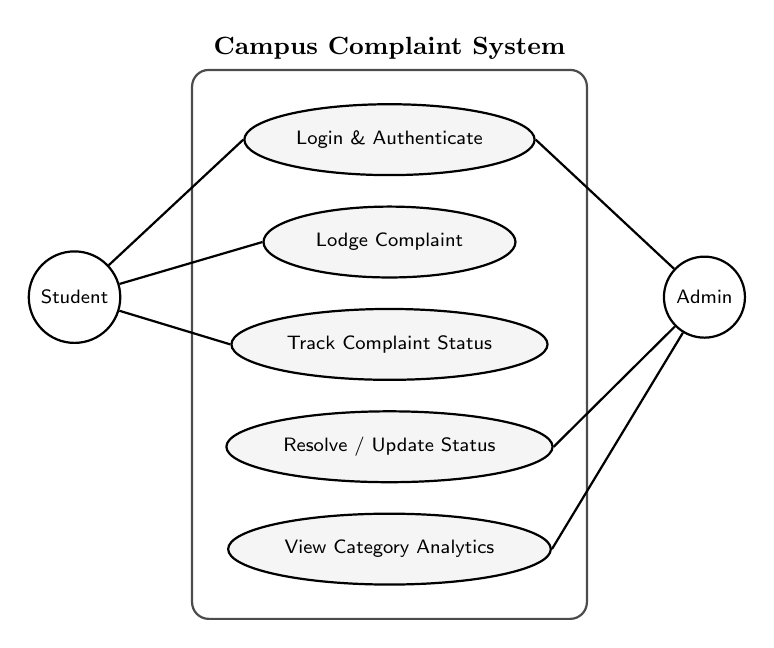
\begin{tikzpicture}[
    actor/.style={circle, draw=black, thick, minimum size=0.8cm, font=\scriptsize\sffamily},
    usecase/.style={ellipse, draw=black, thick, fill=gray!8, align=center, minimum width=3.2cm, minimum height=0.9cm, font=\scriptsize\sffamily},
    boundary/.style={draw=black!70, thick, rounded corners=6pt, inner sep=12pt}
]

% Actors
\node[actor] (student) at (-4, -1.5) {Student};
\node[actor] (admin) at (4, -1.5) {Admin};

% System Boundary and Use Cases
\node[usecase] (uc1) at (0, 0.5) {Login \& Authenticate};
\node[usecase] (uc2) at (0, -0.8) {Lodge Complaint};
\node[usecase] (uc3) at (0, -2.1) {Track Complaint Status};
\node[usecase] (uc4) at (0, -3.4) {Resolve / Update Status};
\node[usecase] (uc5) at (0, -4.7) {View Category Analytics};

\node[boundary, fit=(uc1) (uc2) (uc3) (uc4) (uc5), label=above:{\textbf{\small Campus Complaint System}}] (box) {};

% Associations
\draw[thick] (student) -- (uc1.west);
\draw[thick] (student) -- (uc2.west);
\draw[thick] (student) -- (uc3.west);

\draw[thick] (admin) -- (uc1.east);
\draw[thick] (admin) -- (uc4.east);
\draw[thick] (admin) -- (uc5.east);

\end{tikzpicture}%
}
\caption{UML Use Case Diagram}
\label{fig:use_case}
\end{figure}



\subsection{System Architecture Diagram}
Figure~\ref{fig:arch_diagram} details the layered separation of concerns from the client presentation tier to the persistent storage layer.

\begin{figure}[H]
\centering
\resizebox{0.95\textwidth}{!}{%
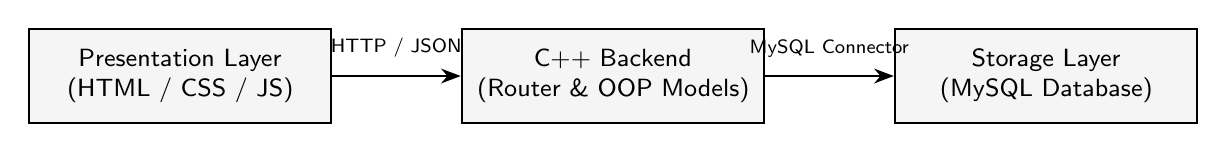
\begin{tikzpicture}[
    block/.style={rectangle, draw=black, thick, fill=gray!8, text width=3.6cm, minimum height=1.2cm, align=center, font=\small\sffamily},
    arrow/.style={-{Stealth[length=2.5mm]}, thick}
]
\node[block] (client) at (0, 0) {Presentation Layer\\(HTML / CSS / JS)};
\node[block] (server) at (5.5, 0) {C++ Backend\\(Router \& OOP Models)};
\node[block] (db) at (11, 0) {Storage Layer\\(MySQL Database)};

\draw[arrow] (client.east) -- (server.west) node[midway, above=3pt, font=\scriptsize\sffamily] {HTTP / JSON};
\draw[arrow] (server.east) -- (db.west) node[midway, above=3pt, font=\scriptsize\sffamily] {MySQL Connector};
\end{tikzpicture}%
}
\caption{System Architecture Overview}
\label{fig:arch_diagram}
\end{figure}

\subsection{UML Class Diagram}
Figure~\ref{fig:uml_class} illustrates the primary class hierarchy, inheritance trees, and class dependencies.

\begin{figure}[H]
\centering
\resizebox{\textwidth}{!}{%
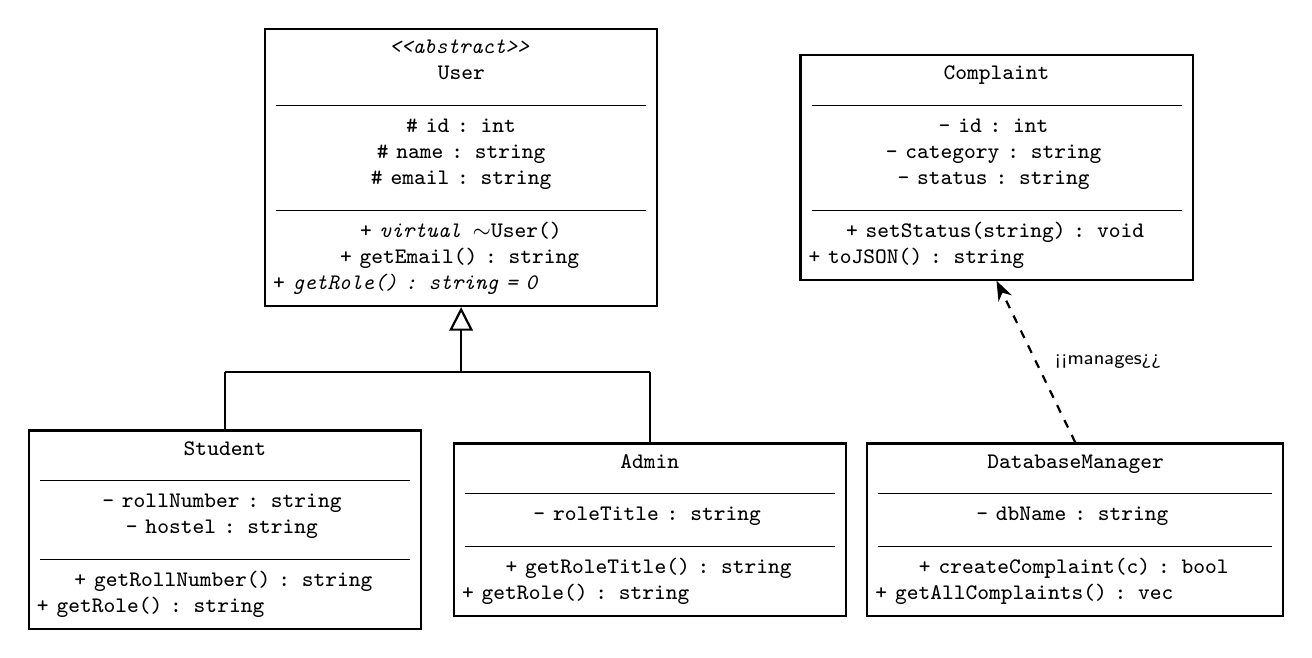
\begin{tikzpicture}[
    umlclass/.style={rectangle, draw=black, thick, fill=white, text width=4.7cm, align=left, font=\footnotesize\ttfamily, inner sep=4pt},
    inherit/.style={-{Triangle[open, length=3mm, width=3mm]}, thick},
    depend/.style={-{Stealth[length=2.5mm]}, thick, dashed}
]

% Top Row: Abstract User and Complaint
\node[umlclass] (User) at (0, 0) {
    \centering\textbf{\textit{<<abstract>>}}\\ \textbf{User}\par
    \rule{\linewidth}{0.4pt}
    \# id : int\\ \# name : string\\ \# email : string\\
    \rule{\linewidth}{0.4pt}
    + \textit{virtual} $\sim$User()\\ + getEmail() : string\\ + \textit{getRole() : string = 0}
};

\node[umlclass] (Complaint) at (6.8, 0) {
    \centering\textbf{Complaint}\par
    \rule{\linewidth}{0.4pt}
    - id : int\\ - category : string\\ - status : string\\
    \rule{\linewidth}{0.4pt}
    + setStatus(string) : void\\ + toJSON() : string
};

% Bottom Row: Concrete Roles and Manager
\node[umlclass] (Student) at (-3.0, -4.6) {
    \centering\textbf{Student}\par
    \rule{\linewidth}{0.4pt}
    - rollNumber : string\\ - hostel : string\\
    \rule{\linewidth}{0.4pt}
    + getRollNumber() : string\\ + getRole() : string
};

\node[umlclass] (Admin) at (2.4, -4.6) {
    \centering\textbf{Admin}\par
    \rule{\linewidth}{0.4pt}
    - roleTitle : string\\
    \rule{\linewidth}{0.4pt}
    + getRoleTitle() : string\\ + getRole() : string
};

\node[umlclass, text width=5.0cm] (DBMgr) at (7.8, -4.6) {
    \centering\textbf{DatabaseManager}\par
    \rule{\linewidth}{0.4pt}
    - dbName : string\\
    \rule{\linewidth}{0.4pt}
    + createComplaint(c) : bool\\ + getAllComplaints() : vec
};

% Standard UML Generalization Tree (No Collisions)
\draw[inherit] (0, -2.6) -- (User.south);
\draw[thick] (-3.0, -2.6) -- (2.4, -2.6);
\draw[thick] (-3.0, -2.6) -- (Student.north);
\draw[thick] (2.4, -2.6) -- (Admin.north);

% Dependency Arrow to Complaint
\draw[depend] (DBMgr.north) -- (Complaint.south) node[midway, right=3pt, font=\scriptsize\sffamily] {<<manages>>};

\end{tikzpicture}%
}
\caption{UML Class Diagram for Domain Models}
\label{fig:uml_class}
\end{figure}

\subsection{UML Sequence Diagram}
Figure~\ref{fig:seq_diagram} traces message passing and object invocation during complaint submission.

\begin{figure}[H]
\centering
\resizebox{0.9\textwidth}{!}{%
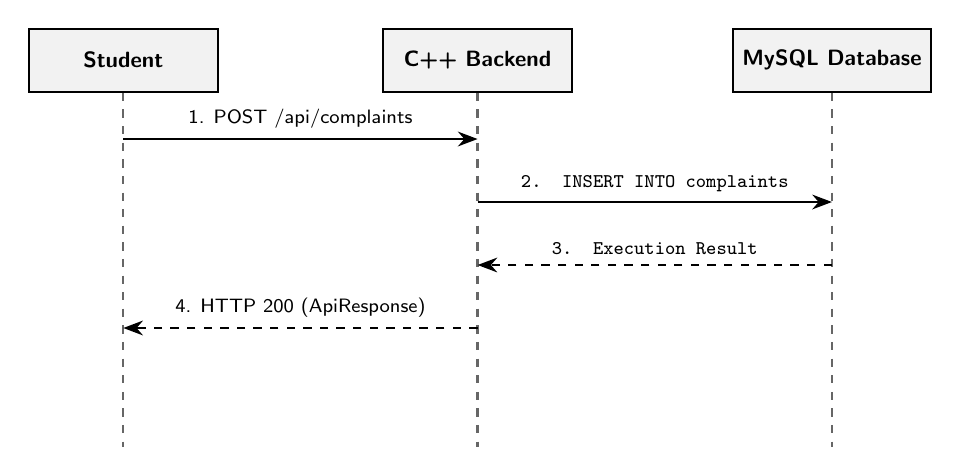
\begin{tikzpicture}[
    participant/.style={rectangle, draw=black, thick, fill=gray!10, minimum width=2.4cm, minimum height=0.8cm, align=center, font=\footnotesize\sffamily\bfseries},
    lifeline/.style={dashed, thick, draw=black!60},
    msg/.style={-{Stealth[length=2.5mm]}, thick},
    ret/.style={-{Stealth[length=2.5mm]}, thick, dashed}
]
\node[participant] (S) at (0,0) {Student};
\node[participant] (BE) at (4.5,0) {C++ Backend};
\node[participant] (DB) at (9,0) {MySQL Database};

\draw[lifeline] (S.south) -- ++(0,-4.5);
\draw[lifeline] (BE.south) -- ++(0,-4.5);
\draw[lifeline] (DB.south) -- ++(0,-4.5);

\draw[msg] (0,-1.0) -- (4.5,-1.0) node[midway, above, font=\scriptsize\sffamily] {1. POST /api/complaints};
\draw[msg] (4.5,-1.8) -- (9.0,-1.8) node[midway, above, font=\scriptsize\ttfamily] {2. INSERT INTO complaints};
\draw[ret] (9.0,-2.6) -- (4.5,-2.6) node[midway, above, font=\scriptsize\ttfamily] {3. Execution Result};
\draw[ret] (4.5,-3.4) -- (0,-3.4) node[midway, above, font=\scriptsize\sffamily] {4. HTTP 200 (ApiResponse)};
\end{tikzpicture}%
}
\caption{Sequence Diagram: Complaint Submission Flow}
\label{fig:seq_diagram}
\end{figure}

% ---------------------------------------------------------
% CODE SNIPPETS SECTION
% ---------------------------------------------------------
\section{OOP Implementation Code Snippets}

\subsection{Inheritance and Polymorphism}
Listing~\ref{lst:inheritance} demonstrates dynamic polymorphism using an abstract base class with pure virtual methods.

\begin{lstlisting}[caption={Inheritance Hierarchy for User Roles}, label={lst:inheritance}]
class User {
protected:
    int id;
    std::string name;
    std::string email;
public:
    User(int i, std::string n, std::string e) : id(i), name(n), email(e) {}
    virtual ~User() = default;
    
    // Pure virtual method enforcing runtime polymorphism
    virtual std::string getRole() const = 0; 
};

class Student : public User {
private:
    std::string rollNumber;
public:
    Student(int i, std::string n, std::string e, std::string roll) 
        : User(i, n, e), rollNumber(roll) {}

    std::string getRole() const override {
        return "STUDENT";
    }
};
\end{lstlisting}

\subsection{Generic Programming and Operator Overloading}
Listing~\ref{lst:template} showcases generic response structuring and stream output serialization.

\begin{lstlisting}[caption={Generic ApiResponse Template and Operator Overloading}, label={lst:template}]
template <typename T>
class ApiResponse {
private:
    bool success;
    std::string message;
    T data;
public:
    ApiResponse(bool s, std::string m, T d) : success(s), message(m), data(d) {}

    // Overloaded stream operator for output formatting
    friend std::ostream& operator<<(std::ostream& os, const ApiResponse<T>& res) {
        os << "[Response] Status: " << (res.success ? "OK" : "ERROR")
           << " | Message: " << res.message;
        return os;
    }
};
\end{lstlisting}

% ---------------------------------------------------------
% PROJECT SCREENSHOTS SECTION
% ---------------------------------------------------------
\section{Project Screenshots and User Interface}
The screenshots below show the frontend interface communicating with the C++ backend services.

\begin{figure}[H]
    \centering
    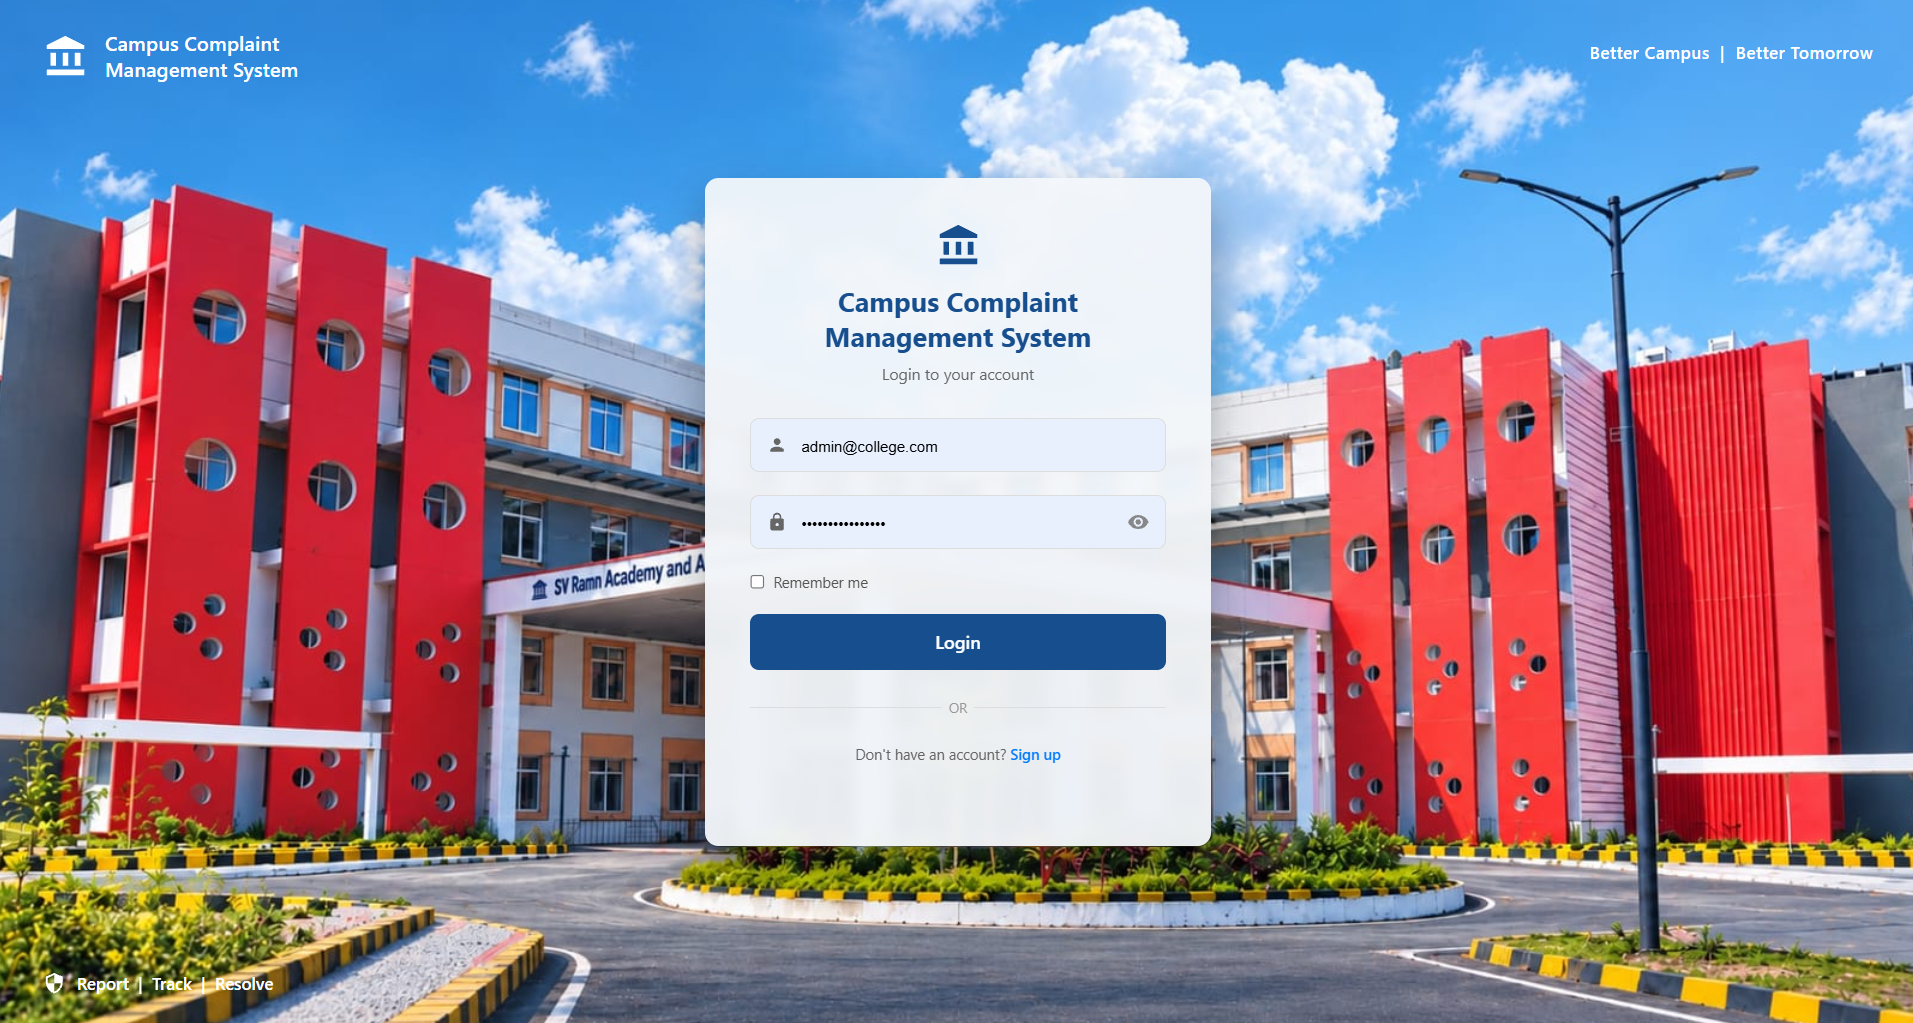
\includegraphics[width=0.85\textwidth]{login}
    \caption{Unified Authentication Portal}
    \label{fig:login}
\end{figure}

\begin{figure}[H]
    \centering
    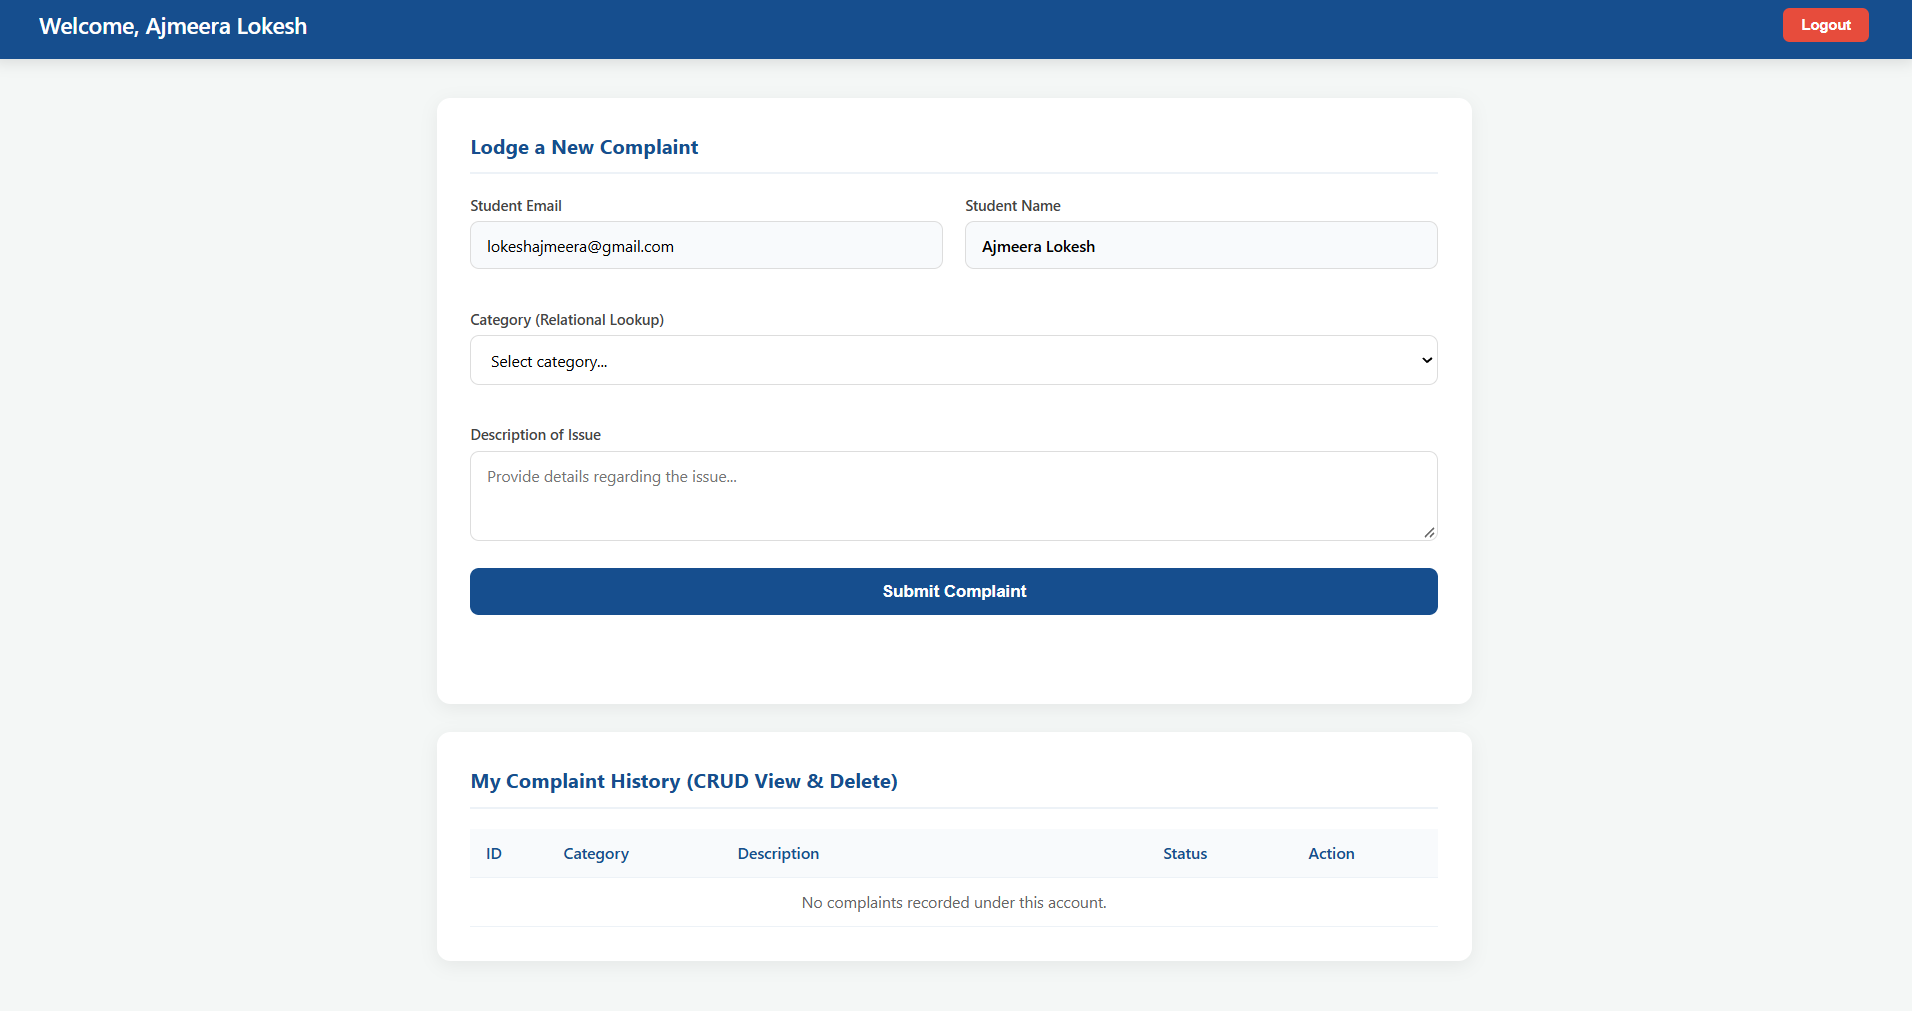
\includegraphics[width=0.85\textwidth]{student_dashboard}
    \caption{Student Dashboard: Grievance Submission and History Tracking}
    \label{fig:student_dash}
\end{figure}

\begin{figure}[H]
    \centering
    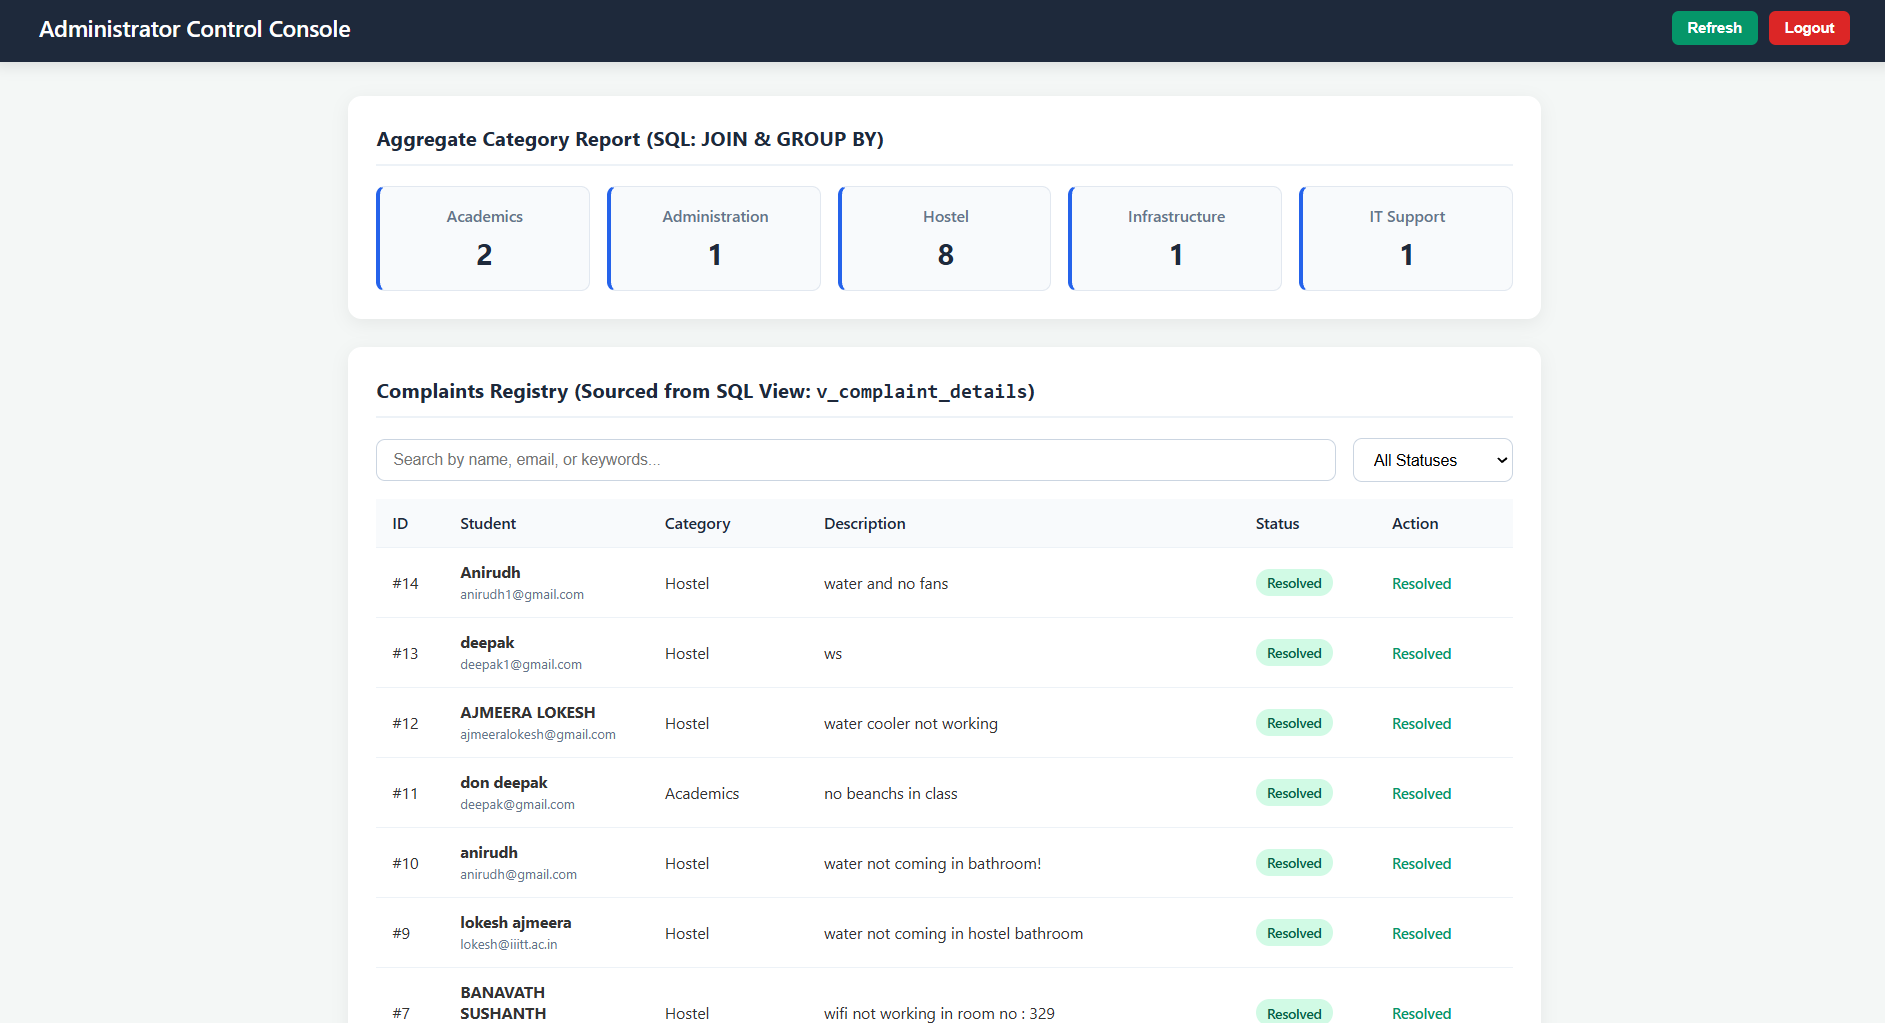
\includegraphics[width=0.85\textwidth]{admin_dashboard}
    \caption{Administrator Control Console: Aggregate Metrics and Complaint Registry}
    \label{fig:admin_dash}
\end{figure}

\end{document}
